\documentclass[11pt,a4paper]{article}

% Packages
\usepackage[utf8]{inputenc}
\usepackage[T1]{fontenc}
\usepackage[margin=1in]{geometry}
\usepackage{mathpazo} % Elegant font
\usepackage{microtype}
\usepackage{xcolor}
\usepackage{graphicx}
\usepackage{booktabs}
\usepackage{multicol}
\usepackage{enumitem}
\usepackage{titlesec}
\usepackage[hidelinks]{hyperref}
\usepackage{float}
\usepackage{subcaption}
\usepackage{caption}
\captionsetup[figure]{labelfont=bf, font=small, textfont=it, labelsep=period}

% Colors
\definecolor{primary}{RGB}{0, 83, 156}
\definecolor{secondary}{RGB}{60, 60, 60}
\definecolor{figurebg}{RGB}{245, 245, 245}

% Title formatting
\titleformat{\section}{\color{primary}\Large\bfseries\sffamily}{\thesection}{1em}{}
\titleformat{\subsection}{\color{secondary}\normalsize\bfseries\sffamily}{\thesubsection}{1em}{}
\renewcommand{\thesection}{\Roman{section}}

% List spacing
\setlist[itemize]{leftmargin=1.5em, topsep=0.2em}
\setlist[enumerate]{leftmargin=1.5em, topsep=0.2em}
% Document metadata
\title{\textbf{\textcolor{primary}{Store and SKU Conversion Analysis Summary}}}
\author{\textbf{Md Kaif} \\ \href{https://github.com/yourusername/your-repo}{\textcolor{primary}{GitHub Project Link}}}
\date{\small\today}

\begin{document}

\maketitle

\section*{Key Findings}

\begin{enumerate}
    \item \textbf{Performance Disparity}
    \begin{itemize}
        \item Store conversion rates range from \textbf{34.6\% (Store\_15)} to \textbf{66.5\% (Store\_39)}.
        \item SKU conversion rates vary between \textbf{41.8\% (SKU\_12)} and \textbf{58.6\% (SKU\_11)}, highlighting consistent high-performers.
    \end{itemize}

    \item \textbf{Top Performers}
    \begin{itemize}
        \item Stores: \textbf{Store\_39 (66.5\%)}, \textbf{Store\_49 (64.6\%)}, and \textbf{Store\_44 (63.1\%)}
        \item SKUs: \textbf{SKU\_11 (58.6\%)}, \textbf{SKU\_7 (56.1\%)}, \textbf{SKU\_16 (54.8\%)}
    \end{itemize}

    \item \textbf{Underperformers}
    \begin{itemize}
        \item Stores: \textbf{Store\_15 (34.6\%)}, \textbf{Store\_14 (36.5\%)}, \textbf{Store\_36 (37.6\%)}
        \item SKUs: \textbf{SKU\_12 (41.8\%)}, \textbf{SKU\_19 (44.3\%)}, \textbf{SKU\_20 (45.1\%)}
    \end{itemize}

    \item \textbf{Revenue vs. Conversion Mismatch}
    \begin{itemize}
        \item High-revenue SKUs such as \textbf{SKU\_3} have moderate conversion rates.
        \item \textbf{SKU\_10 in Store\_10} had 927 visits with \textbf{0\% conversion}, indicating untapped potential.
    \end{itemize}
\end{enumerate}

\section*{Distribution Analysis}

\begin{figure}[H]
    \colorbox{figurebg}{
    \begin{minipage}{\dimexpr\linewidth-2\fboxsep}
        \centering
        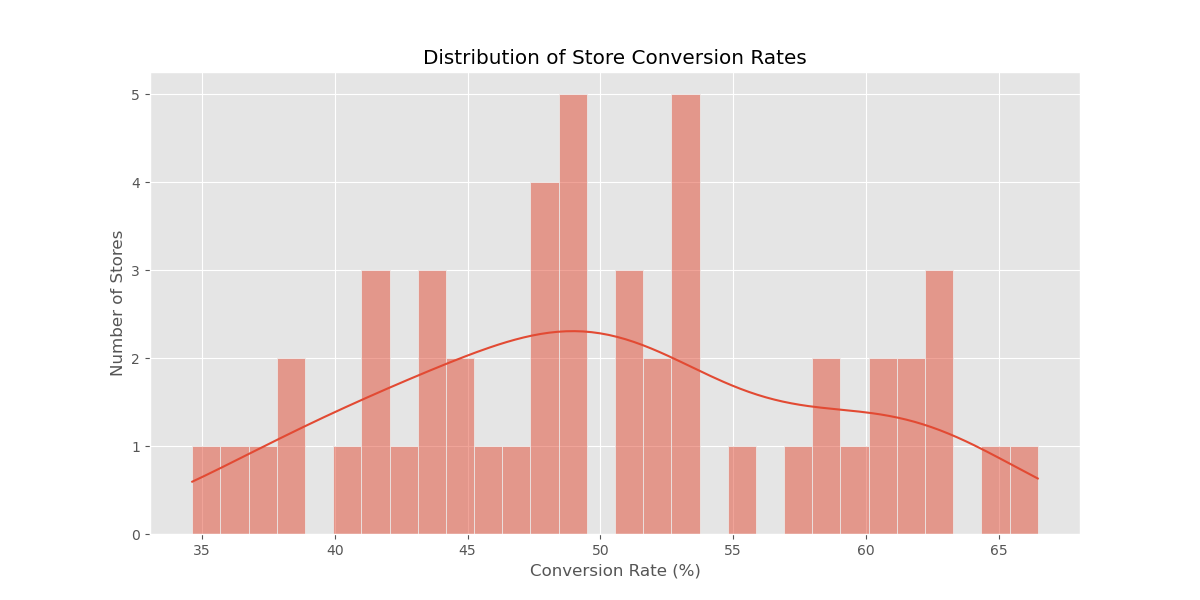
\includegraphics[width=0.9\linewidth]{store_conversion_distribution.png}
        \caption{Distribution of conversion rates across stores}
    \end{minipage}}
\end{figure}

\vspace{1em}

\begin{figure}[H]
    \colorbox{figurebg}{
    \begin{minipage}{\dimexpr\linewidth-2\fboxsep}
        \centering
        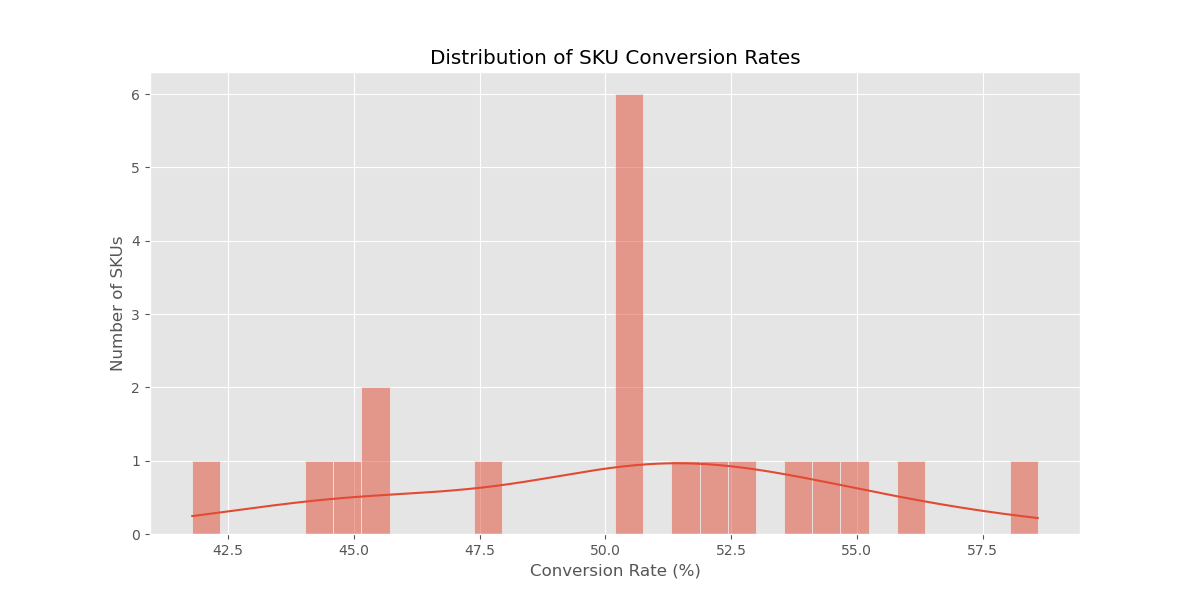
\includegraphics[width=0.9\linewidth]{sku_conversion_distribution.png}
        \caption{Distribution of conversion rates across SKUs}
    \end{minipage}}
\end{figure}

\vspace{1em}

\begin{figure}[H]
    \colorbox{figurebg}{
    \begin{minipage}{\dimexpr\linewidth-2\fboxsep}
        \centering
        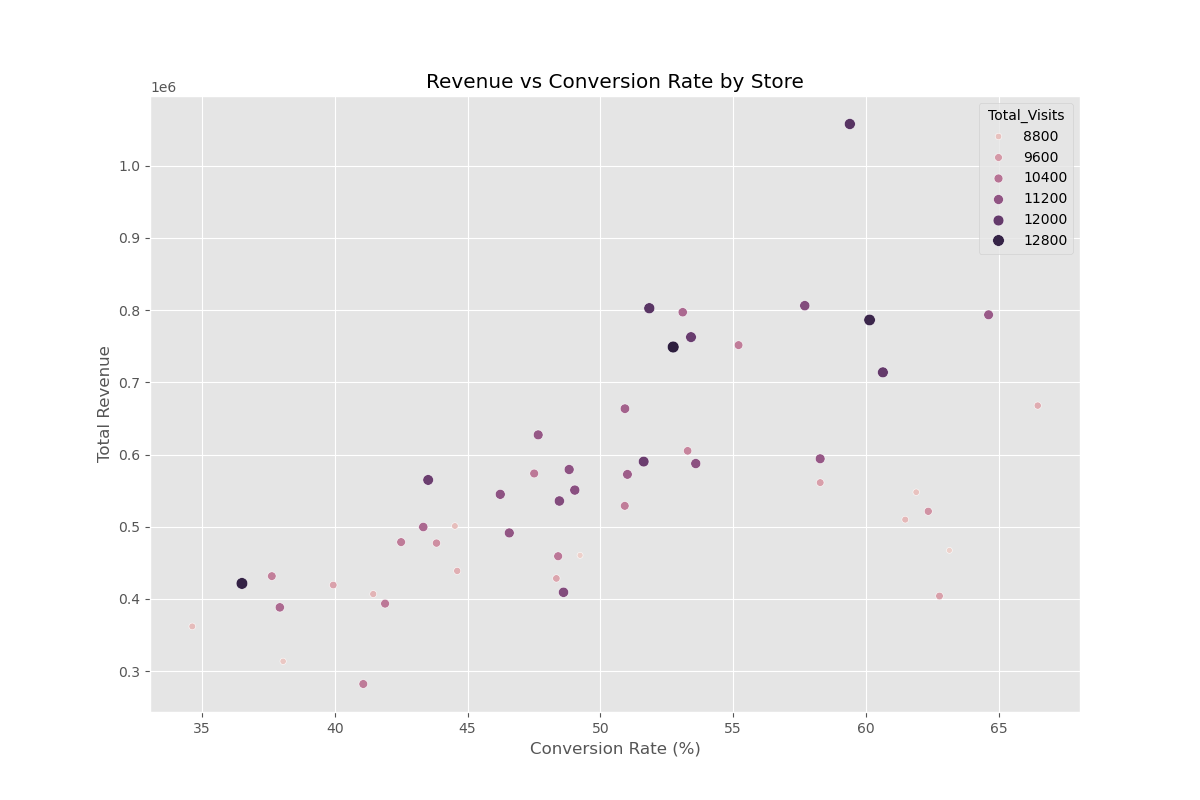
\includegraphics[width=0.85\linewidth]{revenue_vs_conversion_scatter.png}
        \caption{Revenue vs. Conversion Rate by Store}
    \end{minipage}}
\end{figure}

\section*{Recommendations}

\subsection*{1. For Top-Performing Stores}
\begin{itemize}
    \item Share successful strategies such as staff training and store layout optimization.
    \item Expand these practices to new stores for consistency.
\end{itemize}

\subsection*{2. For Underperforming Stores}
\begin{itemize}
    \item Conduct audits to detect inefficiencies (e.g., stockouts or delays).
    \item Provide targeted staff training to enhance customer service.
\end{itemize}

\subsection*{3. For High-Conversion SKUs}
\begin{itemize}
    \item Increase stock availability to prevent missed sales.
    \item Highlight them in promotional campaigns.
\end{itemize}

\subsection*{4. For Low-Conversion SKUs}
\begin{itemize}
    \item Adjust pricing or bundle with better-performing products.
    \item Improve shelf placement in high-traffic zones.
\end{itemize}

\subsection*{5. Data \& Team Enhancements}
\begin{itemize}
    \item Implement real-time monitoring dashboards.
    \item Combine centralized and embedded analytics teams for context-rich insights.
\end{itemize}

\section*{Expected Impact}
\begin{table}[H]
    \centering
    \renewcommand{\arraystretch}{1.3}
    \begin{tabular}{@{}ll@{}}
        \toprule
        \textbf{Metric} & \textbf{Projected Improvement} \\
        \midrule
        Overall Revenue & 15--20\% \\
        Inventory Turnover & 10--15\% \\
        Conversion Rate (Bottom Stores) & 8--12\% \\
        \bottomrule
    \end{tabular}
    \caption{Expected Performance Improvements}
\end{table}

\section*{Next Steps}
Prioritize quick wins (e.g., SKU placement) while developing long-term plans like staff development and inventory realignment.

\end{document}
